\section{写一本给你的量子力学讲义}

100个赞助人,每人100元,众筹万元写一本适合自学的量子力学讲义,款项征集完成后的两个月内完成讲义的写作,并按知识共享-署名(CC-BY)的方式发布在互联网上,我将在讲义中致谢每一位赞助人,同时邀请赞助人加入相应微信/QQ讨论群。

项目发起/执笔人:季燕江,1994年毕业于南京大学物理系理论物理专业,自2002年起在北京科技大学讲授量子力学,自然科学史,量子多体理论等课程。

\begin{figure}[htbp]
\begin{center}
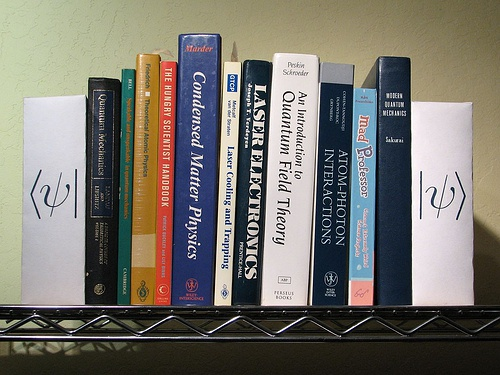
\includegraphics[width=10cm]{Appendix/qmbooks.jpg}
%\caption{default}
%\label{default}
\end{center}
\end{figure}

量子力学是科学家的通用语言,其应用范围早已超越理论物理,侵入到几乎所有科学和技术的领域。作为一门基础和中枢性的理论科学,量子力学的基本概念和术语也渗透到人文和日常的领域,学习量子力学正越来越成为现代人无法回避的任务,我们生活在一个以技术、消费和创意为基础的现代社会,学习量子力学是我们理解今日世界如何运作的必不可少的基础,或如费曼所说:物理学家如何看待世界是真正的现代文化的主要部分。

基于此目的,我将撰写一本适合于每一个现代人自学的量子力学讲义,现征集100个小伙伴支持此计划,每人100元,筹款目标一万元,款项征集完成后的两个月内完成讲义的写作,并按知识共享-署名(CC-BY)的方式发布在互联网上。在我的设想中,这将是一本标准的教材,有习题、解答,自学完成后大致相当于大学物理系本科的水准,同时这又不是一本传统的教材,我将不厌其烦地尝试用多种角度和方式,历史的、哲学的、图像的、比喻的等等去建立和阐释其中伟大的物理。

参与方式:

豆瓣存档:\url{http://site.douban.com/223228/}

【Q\&A】

1.为什么选择众筹的方式完成此计划?

科学研究,文学写作,甚至当代艺术在今天都是高度机制化的,我们必须符合某种规范才能在这个机制中生存,然后才能虚假地谈论我们的自由和理想,这本身就是令人作呕的。众筹使我们直接面对大众,我们的创意通过媒介与潜在的志同道合、心气相通者发生沟通和互动,这使我们获得种种尝试和改变的机会。具体到写作讲义,假使有越来越多的人加入到此类实践中去,形成风气,我们就有更多机会选择,与更多人发生关系、创造新的学习机会并完善我们自己。

2.为什么是量子力学?两个月是否会很仓促?

自2002年秋季起,我就开始在北京科技大学讲授量子力学,这是我最热爱、最熟悉、最喜欢讲授的一门课程。课程使用的讲义也是我自己编写的,很早就分享在互联网上,地址是:\url{http://ishare.iask.sina.com.cn/f/66602364.html}(*爱问共享暂时无法访问)

两个月确实蛮紧张,但我的假设是,一旦开始此计划,我将每天至少为此工作6小时,是全身心的投入,而在筹款期间我将继续做一些准备工作,比如修改提纲,撰写例题和解答等。

3.为什么筹款目标是一万元?

鉴于我将全身心地为此工作两个月时间,鉴于我的教育背景和职业训练,鉴于每个人都需要现实地生活在这个世界上,鉴于你和很多人都可能需要这样一本讲义,一万元是个合适的数额。

4.为什么不选择传统的出版社?

在互联网的时代,知识渴望自由;知识渴望碰撞、融合和变异。今天,凡是提高知识获取门槛,阻碍知识自由传播、研习的行为都是反动、反历史的。对既有反动机制最好的回应方式就是弃绝一切用知识,用写作谋利的机会,把自己的创造物直接存档于网络空间,以待同道。

不通过传统出版,而使用众筹获得的资金进行讲义的写作和修订,实际上是更便宜,更有效率和更值得追求的,成本由赞助者一次性投入,全部支付到写作者手中,而真正受读者欢迎的讲义在未来也将获得更多修订续写的机会。在此意义下,读者和写作者将获得更多的自主和自由。

5.关于量子力学国内外已经有那么多经典教材,我们为什么还需要一本新的讲义?

首先量子力学与我们先前学习过的任何一门科学课都有本质的不同,每个初学者在学习的时候都需要经过一番思想上的搏斗才会颠覆日常概念,建立量子概念,这个思维的过程对我们每个人都是不同的,每一种新讲法、新表述、新途径都有不可替代的价值和意义。其次,量子力学迄今仍然是最有生命力和扩张力的基础理论,它不断地被应用到新的现象和领域,并不断地取得成功,我们应当在讲义中对这些新进展有所体现。

通过浏览国外知名大学的量子力学课程主页,我们会发现迄今一直在不断涌现新的量子力学讲义和课程设计,可以说每个优秀教师都应该有关于量子力学课程的带有自己个人风格的讲法和讲义,这门课程绝非几本经典教材或几套典型教法可以概括。

6.我的数学基础很差,能否学会量子力学?

假设大家具有高中水平的数学知识,我在讲义中将不回避使用数学,不回避使用数学概念,数学公式,推导计算等等。

不回避数学的原因与我所理解的量子力学有关,量子力学缺乏本质,我们不能或很难说量子力学是什么。量子力学是关于表示的,此一特征与所有的文学或艺术类似,我们经由经验或实验获得陈述,这所有的陈述呼唤我们为它们建立起种种表示,这种种表示中有一套或几套数学使我们能够去继续相关的实践或实验探索。不在讲义中使用数学我们就无法了解今日之精密科学,就无法了解今日之实验科学与理论科学间的精妙关联和缠绕。

不回避数学并不就意味着枯燥,我将尽量使用简单、日常的语言引入数学概念,除必不可少、最低限度的数学外,繁复啰嗦的数学推导会作为例题、应用和专论单独处理,完全跳过这些内容将不会妨碍我们继续学习量子力学。

7.这将是一本很轻松的讲义吗?

尽管我的立意是要写一本适合普通人阅读自修的量子力学,但这并不意味着很轻松,研习任何知识都需要真正认真地思考,正如朗道和基泰戈罗茨基在《大众物理学》序言中强调的,“我们并不怜悯读者。如果要弄懂这本书,书中的许多地方只读一遍或两遍是不够的,需要认真地思考。”

8.我有兴趣,通过此计划我能获得什么?

首先我将在讲义中致谢每一位赞助人,感谢大家帮助、激励我实现自己的想法,使这样一本免费共享,符合互联网精神的讲义变为现实。其次我将邀请你加入相应微信/QQ讨论群,我们将通过此微信群长期与大家交流研习量子力学的经验。你可以通过任何渠道向我建议讲义中应当涉及的内容或写作的方式风格等等,当然最终的取舍将完全取决于我。

~~


谢谢!

季燕江(微信号:ianwest;传说中奇迹文库的创建者,如果你不知道,就请忽略吧。)

Open access now, miracle in future!

原始网址:\url{http://www.douban.com/note/328179561/}

